\documentclass[11pt,a4paper]{article}
\usepackage[utf8]{inputenc}
\usepackage{amsmath}
\usepackage{amsfonts}
\usepackage{amssymb}
\usepackage{graphicx}
\usepackage[left=2cm,right=2cm,top=2cm,bottom=2cm]{geometry}
\author{Van Vincent Duong}
\title{Scattering Amplitudes Research Project}
\begin{document}

\maketitle

\section*{Week 1}

Scattering amplitudes are calculated from the fundamental interactions occurring at the quantum scale in collisions.  They are useful in scattering experiments, especially at ultra-relativistic energies.  The research project this summer has a few goals:
\begin{itemize}
	\item Long-tern: 
\end{itemize}

\section*{Week 2}
\subsection*{Readings}
\subsection*{Meetings}
The aim of this project is to constrain the low-energy limit scattering amplitude of 4 gravitons.  This amounts to studying higher derivative corrections to the Einstein-Hilbert action in 3+1 dimensional general relativity:
\begin{align*}
S & = \frac{1}{16\pi G}\int d^4x \sqrt{-g}R.
\end{align*}
But nothing is stopping us from postulating that there are higher order derivative corrections to the full Lagrangian, as long as they are small and covariant.  What does small mean?  Remember that curvature $R$ has units of inverse length squared ($[R] = L^{-2} = M^{2}$), and that Newton's Constant has units of length squared ($[G_N] = M^{-2}$).  So, the action could take the form of
\begin{align*}
S & = \frac{1}{16\pi G}\int d^4x \sqrt{-g}(R + \mathcal{O}(G R^2) + \cdots ).
\end{align*}
The purpose of this exercise is to show how the full Lagrangian can contain additional terms.  In Quantum Field Theory, this directly translates to a new set of Feynman rules and more rich interactions (but perhaps not allowed as we will soon find out!).  New Feynman rules emerge when quantize the gravitational degrees of freedom of the metric tensor $g_{\mu \nu}$.  If we treat gravitons as metric excitation around a flat space-time, then there is a perturbation expansion:

\begin{align*}
	g_{\mu \nu} = \eta _{\mu \nu} + \epsilon h_{\mu \nu}.
\end{align*}
It is precisely the tensor of $h_{\mu \nu}$ which tell us how gravitons emerge in flat-space.

It is also worth asking how can gravitons couple to matter?  For example, a straightforward procedure would be to introducing a scalar particle $\phi$.  In flat space-time, the scalar particle has the following Lagrangian description:
\begin{align*}
	S_{\mathrm{scalar}} = \int d^4 x \left(\partial^\mu \phi \partial_\mu \phi- m^2 \phi^2\right),
\end{align*}
which can be promoted to a covariant action by introducing appropriate measures and derivatives:
\begin{align*}
	S_{\mathrm{scalar}} = \int d^4 x \sqrt{-g}\left(\nabla^\mu \phi \nabla_\mu \phi - m^2 \phi^2\right).
\end{align*}
The game is now to expand the metric using the $\epsilon$ introduced above. 

So how does this all fit together?  The techniques outlined above allow us to better understand how gravitons would be quantized and how they would couple to matter by first postulating the form of the Lagrangian.  The problem is that there are a myriad of constructions that can be postulated, and then the process of describing each theories own Feynman rules would take a tremendous amount of pen and paper.   Instead we will take the following approach:
\begin{enumerate}
	\item Consider \textbf{2-to-2 graviton} scattering.
	\item Construct the possible scattering amplitude $A_4$ from the \textbf{spinor helicity} formalism + \textbf{little-group scaling} + \textbf{dimensional analysis}.
	\item Apply \textbf{Unitarity and Locality} constraints to the amplitude.
\end{enumerate}
If there are intermediate particles emerging in this interaction (i.e., massive propagators), it would be extremely useful to understand how large the mass is.  This is precisely our goal: If there are heavy particles with masses $m_1, m_2 \dots $ created in the scattering process, is there a mass scale $M$ for which we know that $m_1, m_2, \dots  \geq M$?  This would be useful to know.
\textbf{Basic Techniques:}
\begin{itemize}
	\item Constrain the full-form of the amplitude by studying the high energy limit, whereby particles are effectively massless.
	\item Study the amplitude at Planck scale energies: $\sqrt{s} \approx m_{pl}$.
	\item Study the amplitude in intermediate energy scales: between short (heavy) and long (light) time-scales.
	\item Constrain ourselves to $3 + 1$ dimensions.
	\item Couple a pair of gravitons to a generic massive particle with mass $m$ and spin $J$ (this will require intermediate polarizations).
\end{itemize}

Higher derivative terms come at the cost of new massive propagators commonly of the form:
\begin{align*}
	G(p) \sim \frac{1}{p^2 - m^2}.
\end{align*}
These propagators are directly associated to the force experienced between the two particles via the potential.  Indeed, the propagator is the Fourier transform of the potential $V(r)$:
\begin{align*}
	\int d^4 x e^{-ip\cdot x}V(r) \sim G(p).
\end{align*}
At large impact parameters, the amplitude will reveal the "classical" force.  For example, in the COM of a graviton, the propagator for will be of the form
\begin{align*}
	G(p) \sim \frac{1}{p^2 - m^2} \sim \frac{1}{\vec{p}^2} \implies V(r) \sim \frac{1}{r}.
\end{align*}
It is surprising that classically, the amplitude is invariant whether potential is attractive or repulsive.  That is, the sign of the propagator does not change the experiment.  However, this is not true in the field theoretic picture, in which new Feynman diagrams can interfere (at loop level).  For example, there can exist a relative sign between the following two diagrams:

\begin{figure}[ht]
    \centering
    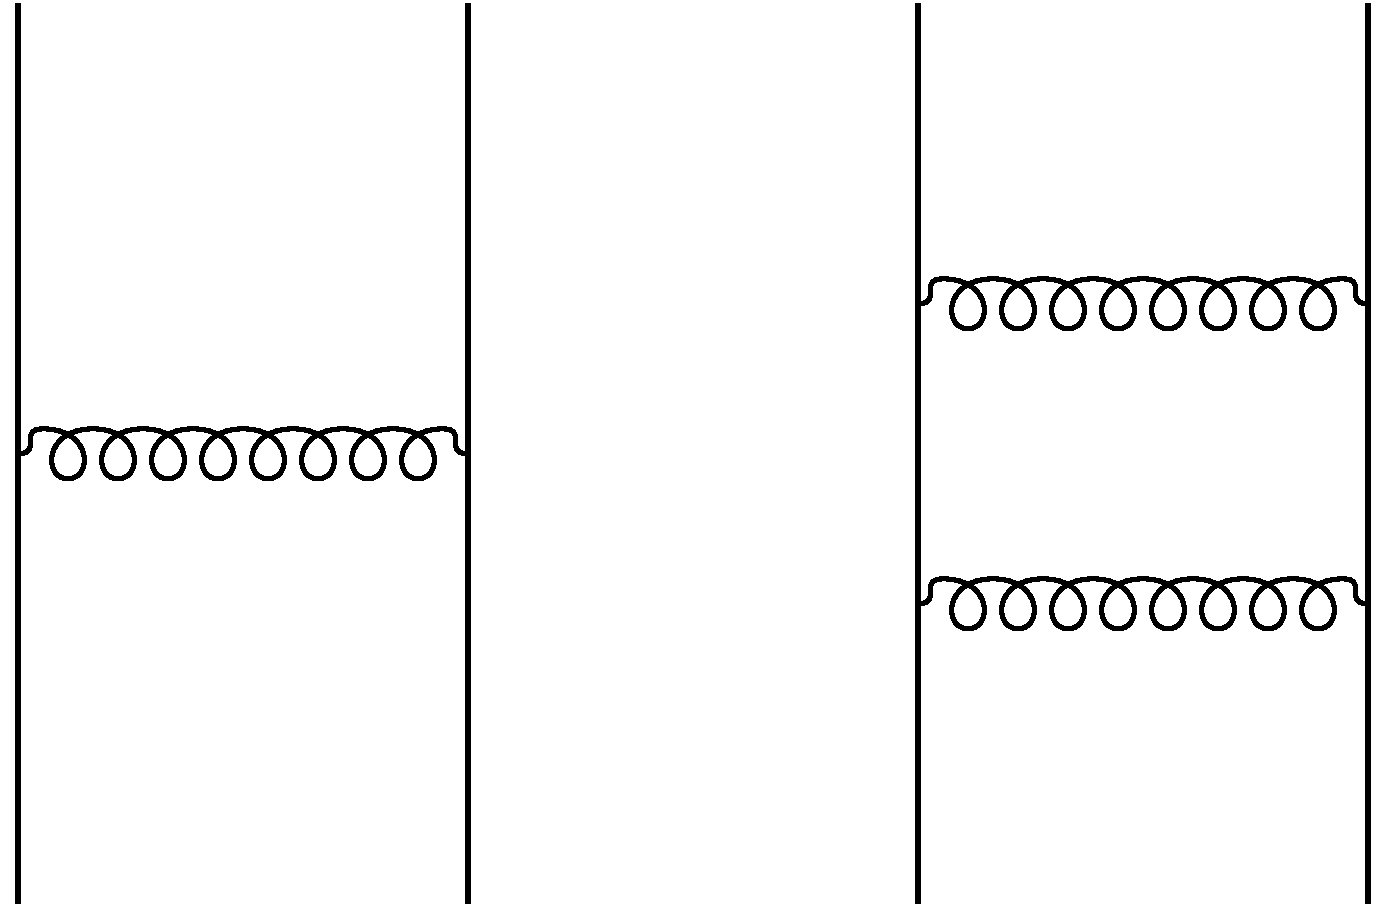
\includegraphics[width=0.3\textwidth]{figures/relative_sign.pdf}
    \caption{Comparison of two Feynman diagrams for the same scattering process.  If propagator carries a negative sign, then there can be a relative negative sign that appears when summing the amplitude from all processes. \textbf{So what?}  The amplitude will interfere and we can discern whether the potential is attractive or repulsive.  However, this comes at a cost: we needed to introduce a loop-level correction!}
    \label{fig:mesh1}
\end{figure}


Bootstrapping the $S$ matrix is the next step.  We define the $S$ matrix by
\begin{align*}
	|f\rangle = \overbrace{(1 + i \mathcal M)}^{S} |i\rangle.
\end{align*}
It is infinite time-evolution operator between initial and final states in a scattering process.  It must therefore be unitary, which means $S$ is hermitian:
\begin{align*}
	S = S^{\dagger}.
\end{align*}
We can also interpret $S$ as a the exponential of the Hamiltonian from standard quantum mechanics
\begin{align*}
S = e^{-i \int dt H} & = 1 - i \int dt \overbrace{H}^{H_0 + V} + \mathcal{O}(H^2) = 1 + i \mathcal{M}\\
\implies \int dt V & = - \mathcal{M}.
\end{align*}

If the potential is attractive, $V < 0$, so that $\mathcal{M} > 0$.  This is a grand result!

Let's now consider a massive propagator. We can extract the underlying force via a Fourier transform:
\begin{align*}
G(p) & \sim \frac{1}{p^2 - m^2}\\
\implies V(r) & \sim \frac{e^{- m r}}{r}.
\end{align*}
There is a characteristic length scale of $1/m$ which emerges when introducing a mass scale $m$.  Let's now consider an interesting case for the 2-to-2 scattering with an intermediate heavy particle:
\begin{figure}[ht]
    \centering
    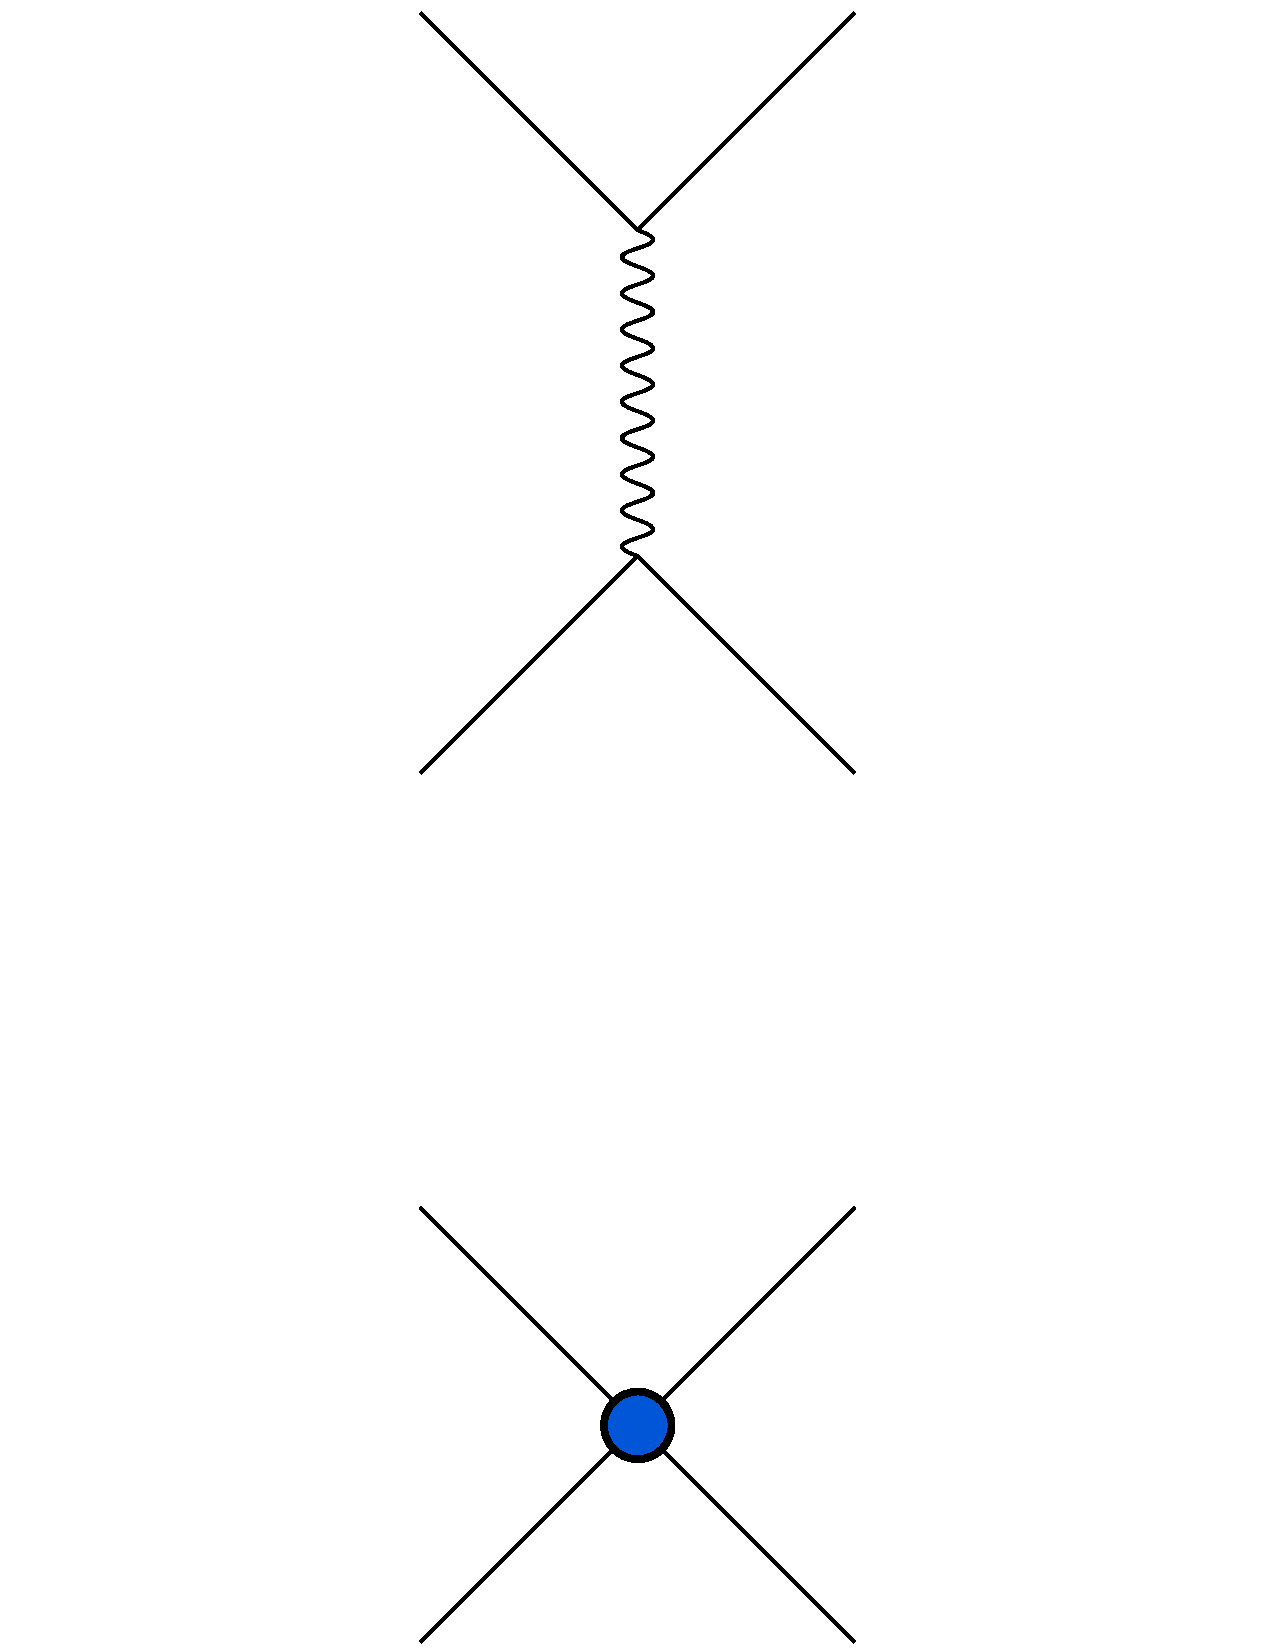
\includegraphics[width=0.3\textwidth]{figures/short_length.pdf}
    \caption{If there is a massive propagator, the interaction essentially collapses from 2 3-point couplings into one 4-point coupling.}
    \label{fig:mesh2}
\end{figure}
It is therefore natural to examine how massive propagators look like as an expansion in $1/m^2$.  For example
\begin{align*}
	G(p) \sim \frac{1}{p^2 - m^2} \approx \frac{1}{m^2}\left(1 - \frac{p^2}{m^2} + \mathcal{O}(p^4/m^4)\right).
\end{align*}
The propagator us now a polynomial expansion in $p$.  We know from Fourier analysis that this corresponds to a $\delta$ potential in position space and leads to the appropriate Feynman rules for higher order derivative terms.
\textbf{Question to answer:} Suppose we find a polynomial correction to the propagator.
\begin{itemize}
	\item Can we find the mass cut-off of the theory $M$?
	\item How does this look like if we are agnostic about the coupling constants in the theory?  They may be small, and have \textit{any} sign.
\end{itemize}
Problem statement:  If we consider 2-to-2 particle scattering with a massive intermediate spin-$J$ particle, what can be said about the amplitude?  There are some complications and general strategies.  The first is to map spin-$J$ particles to polarization 3-vectors.  We need to construct Lorentz invariant quantities such as the vertex rule: $f(\epsilon \cdot v, \epsilon^2, v^2)$. In particular, we can form the intermediate particle of mass $M$ by colliding two gravitons with 4-momenta $M/2 (1,\hat{v}), M/2(1,-\hat{v})$ and the polarization vector $\epsilon$.  Nima found that
\begin{align*}
	A_4 = g^2 \frac{P_J(\cos(\theta_{v,v'}))}{M^2 - s},
\end{align*}
where $P_J$ are the Lagendre polynomials and the angle $\theta_{v,v'}$ denotes one of the angles between in-coming and out-going gravitons

\section*{Week 3}
\subsection*{Readings}
\subsection*{Meetings}
On Tuesday's meeting, we briefly discussed the polarization vectors.  The main discussion revolved around Simon's current work.  I had some confusion on polarization vectors -- they do not transform as a 4-vector and are not well defined when pointing along the direction of motion.  In particular, a spin $J$ particle, will be described by a $2J$ tensor.  For example, they can be described by fields with $A_{\mu_1, \cdots, \mu_{2J}}$.  In QED, these are the usual $\epsilon^{\mu}$ and for a graviton $h_{\mu \nu}$.  
\begin{align*}
	h_{\mu \nu} = \begin{pmatrix}
* & * & *\\ 
 &  * & *\\ 
 &  &  *
\end{pmatrix}.
\end{align*}
There are some constraints: it must be symmetric in its indices because of rotational invariance.  Moreover, it must be traceless.  Thus, the dimensionality for this group should be $\frac{3(3+1)}{2} - 1 = 5 = 2(2) + 1 = 2J + 1$. 
\\
\textbf{Goals for this week}
\begin{itemize}
	\item Read notes from Simon.
	\item Try to enumerate all the possible expansions for the symmetric polynomials to higher order (e.g., $g_4, \cdots$).
	\item Reproduce Simon's work
	\item Familiarize myself with Legendre polynomials and Gegenabaum polynomials.
	\item Notice that eq. 5.41 does \textbf{not} contain gravity while eq. 5.40 does.  Can this be reproduced at higher order corrections?
	\item Can we obtain a bound on the couplings that are independent of $G_N$? That is, can we obtain a universal bound?
\end{itemize}

\subsection*{Notes}
Equation 5.34 of Simon's work claimed that the amplitude from the 2-to-2 scattering of a \textbf{massless} scalar particle can be expanded
\begin{align*}
\mathcal{M}_{\mathrm{low}}(s, t)=& 8 \pi G_{N}\left[\frac{s t}{u}+\frac{s u}{t}+\frac{t u}{s}\right]-g^{2}\left[\frac{1}{s}+\frac{1}{t}+\frac{1}{u}\right]-\lambda \\
&+g_{2}\left(s^{2}+t^{2}+u^{2}\right)+g_{3} s t u+g_{4}\left(s^{2}+t^{2}+u^{2}\right)^{2}+\ldots.
\end{align*}
There are several things I do not understand completely in this Ansatz:
\begin{itemize}
	\item Why does gravity couple only in interactions of the form: $\frac{st}{u}$?  Is this from dimensional analysis?
	\item Why should we expect the expansion to be symmetric in the Mandelstem variables $s,t,u$?  Is this a result from crossing symmetry for scalar particle? \textbf{I can probably show this}
	\item In math, we learn that there is a more natural basis of symmetric polynomials of $3$ variables.  Why are they not used?
\end{itemize}
Simon's equation can be re-written in terms of the natural symmetric polynomials:
\begin{align*}
	e_0 & = 1\\
	e_1 & = s + t + u = 0\\
	e_2 & = st + su + ut\\
	e_3 & = stu
\end{align*}
We will see that the massless condition provides a huge simplification when constructing symmetric polynomials in terms of these basis functions.  I will not re-write Simon's expansion in terms of these basis polynomials
\begin{align*}
	s^2 + t^2 + u^2 & = (s+t+u)^2 - 2(st + su + tu) = e_1 ^2 -2e_2 = -2e_2\\
	(s^2 + t^2 + u^2 )^2 & = 4e_2 ^4.
\end{align*}
This translates to
\begin{align*}
\mathcal{M}_{\mathrm{low}}(s, t)=& 8 \pi G_{N}\left[\frac{s t}{u}+\frac{s u}{t}+\frac{t u}{s}\right]-g^{2}\left[\frac{1}{s}+\frac{1}{t}+\frac{1}{u}\right]-\lambda \\
&+g_{2}\left(-2e_2 ^2 \right)+g_{3} (e_3) +g_{4}\left(4e_2 ^4\right)+\ldots.
\end{align*}
It is now easy to perform a symmetric polynomial expansion of the amplitude in terms of $e_1, e_2, e_3$ order by order.  Each order in the expansion will contain terms that are products of the elementary symmetric polynomials.  Let's check this with the next leading order
\begin{align*}
\mathcal{O}(5) &: \underbrace{e_1^5}_{0}, \underbrace{e_1^3}_{0} e_2, \underbrace{e_1}_{0} e_2 ^2 , \underbrace{e_1^2}_{0}e_3 , e_2 e_3
\end{align*}
\textbf{So what:} the only non-vanishing terms contain powers of $e_2$ and $e_3$ only!  I am now ready to perform the power expansion using the basis of non-vanishing symmetric polynomials.  To adhere with Simon's convention, let us redefine our basis polynomials:
\begin{align*}
	e_2 \rightarrow - \frac{e_2}{2} = s^2 + t^2 + u^2.
\end{align*}
Then computing the expansion:
\begin{align*}
	& g_5 (e_2 e_1)\\
	& g_6 (e_3 ^2) + g_6 '(e_2 ^3)\\
	& g_7 (e_2^2 e_3)\\
	& g_8 (e_3^2 e_2) + g_8 '(e_2 ^4)\\
	& g_9 (e_3^3) + g_9 ' (e_2 ^3 e_3)\\
	&\vdots
\end{align*}
It becomes clear that in the $\mathcal{O}(n)$ order, I will have terms of the form:
\begin{align*}
e_2 ^x e_3 ^y,
\end{align*}
such that $2x + 3y = n$, where $x,y, \in \{0,1,2,\dots\}$.  Moreover, the number of terms at that order will be the number of non-negative solutions for $(x,y)$ that solve the constraint.  
\\
\\
I am now ready to obtain various constraints by appropriately setting either $s,t,u$ to $0$ and checking how things look like.  For example, at order 5:
\begin{align*}
	\frac{1}{s(s+u)}g_5 (stu) (s^2 + t^2 + u^2)& = g_5 \frac{-s(s+u)u}{s (s+u)} (s^2 + (-s-u)^2 + u^2)\\
	& = -g_5 u (s^2 + s^2 + 2us + u^2 + u^2)\\
	& = -2 g_5 u (s^2 + us + u^2)\\
	& \rightarrow -2g_5 u^3 \quad \text{as} \quad s\rightarrow 0\\
	\frac{1}{(st)^2}g_5 (stu) (s^2 + t^2 + u^2)& = g_5 \frac{u}{st}\left(s^2 + t^2 + (-s-t)^2\right)\\
	& =-  2g_5 \frac{s+t}{st}\left(s^2 + st + t^2\right)\\
	& = -2g_5 \left(\frac{1}{t} + \frac{1}{s}\right)\left(s^2 + st + t^2\right)\\
	& = -2g_5 \left(\frac{s^2}{t} + 2s + 2t + \frac{t^2}{s}\right)\\
	& = -2g_5 \left( \frac{s^2}{-(s+u)} + 2s - 2(s+u) + \frac{(s+u)^2}{s}\right)\\
	& \rightarrow -2g_5 \frac{u^2}{s} \quad \text{as} \quad s\rightarrow 0
\end{align*}
\end{document}